\chapter{Multi-Rotor Development}
\label{chap:MR}
\section{Range \& Endurance}
For a multirotor, range can be estimated by how far it can be controlled by the controller before losing its connection. The range of a multirotor is dependent on certain factors like weight, motor power, weather conditions, etc. Based on the application requirement, they can be customized for longer ranges and better performances. In this project, the forward flight momentum theory was used to estimate the range and endurance of the aircraft for a given set of forward speeds. A velocity range of 0-20 m/s was chosen to perform this calculation and the estimated values of range, endurance, and forward speeds of the multi-rotor drone were calculated using the following steps as follows: \\\

\subsection{Forward Flight Momentum Theory}

The forward flight expression can be written as:

\begin{equation}
	\label{eq:range_multirotor}
	v = \frac{T}{2} 
\end{equation}

At a given forward speed, V we can then solve for $ α_D $, v, T, $ P_{ind} $, $ P_{tot} $ as follows: \\\

\begin{enumerate}
	\item Calculate the quadrotor drag $ D = \frac{\rho C_D V^2}{2} $ at $ α_D = 0 $ Assume $ α_D $ does not affect the drag, otherwise need to iterate to find solution
	\item Solve $ α_D = tan^-1(\frac{D}{W}) $
	\item Square both sides of \ref{eq:range_multirotor} replace $ T_2 $ by $ W_2 $ + $ D_2 $ and re-arrange to get, $ v_4 + (2 V sin(α_D)) v_3 + V 2 v_2 −(W2 + D2)/(2 ρ A)2 = 0 $
	\item Positive real root of equation gives v, then $ P_{ind} = T_v; P_{tot} = T (v + V sin(α_D)) $
	\item Notice that this total power does not include profile drag, swirl, or additional
	losses due to non-uniform induced velocity.
	\item Solve for a range of speeds and plot results versus V
		
\end{enumerate}

The maximum range of the quadcopter is calculated using the formula: \\

Max. Range = $ (\frac{E_b * m_e * esc_e }{Minimum Total Power/Velocity}) $ \\

Where, $ E_b $  = Energy of the battery;  $ M_e $ = Motor efficiency;  $ Esc_e $ = ESC efficiency \\

The maximum endurance of the quadcopter is calculated using the formula: \\

Max. Endurance = $ (E_b * m_e * esc_e) / (Minimum Total Power) $ \\
Where, $ E_b $ = Energy of the battery; $ M_e $ = Motor efficiency; $ Esc_e $ = ESC efficiency \\

Based on the above-mentioned procedures, the results of the multi-rotor drone (quadcopter) are as follows: \\
\begin{itemize}
	\item Max. Range = 34 kms
	\item Max. Endurance = 68.1 minutes
	\item Forward Speed for range = 9.5 m/s
	\item Forward Speed for endurance = 7 m/s
\end{itemize}

\section{Quadrotor Dynamics Model}

The development of dynamics model of quadrotor was done by using the following state space matrices given for each control channel.

\textbf{Given State-Space Matrices} : \\
\begin{figure}
	\centering
	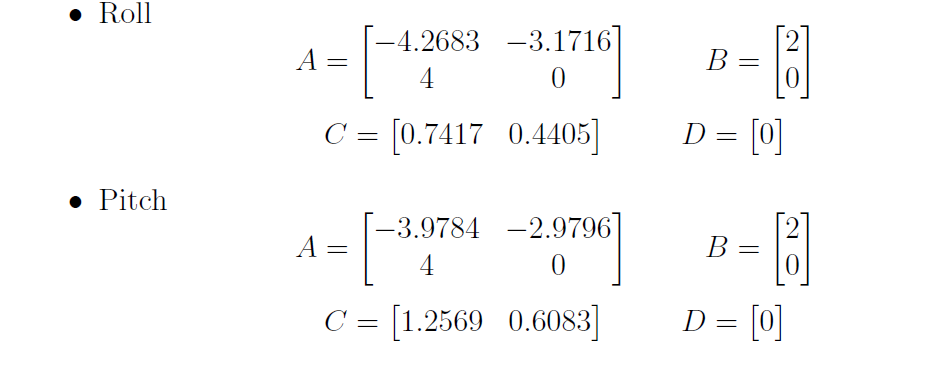
\includegraphics[width=0.8\textwidth]{Images/ss_1}
	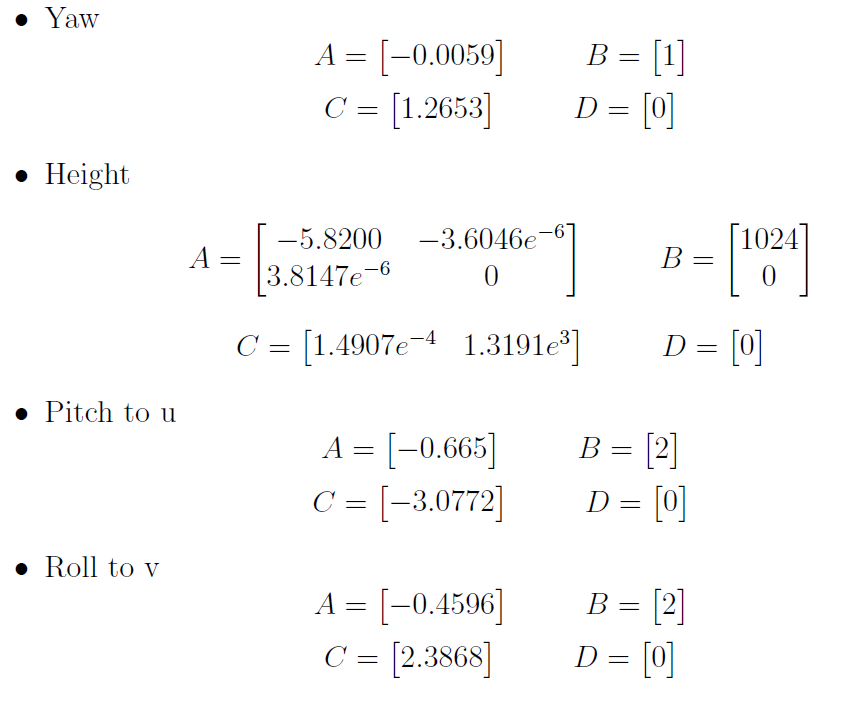
\includegraphics[width=0.8\textwidth]{Images/ss_2}
	\caption{State-Space Matrices}
	\label{fig:ss}
\end{figure}

The output from position controller was fed into the dynamics model. The dynamics model consists of each control channel mentioned above put in a separate state-space block in Simulink. For roll control the input was the desired roll angle and the output from the state-space block was the actual roll angle. This actual roll angle was then fed into the roll to v control channel as input, to get the actual velocity v about y-axis.

For pitch control the input was desired pitch angle and the output was the actual pitch angle. This actual pitch angle was then fed into the pitch to u control channel which gives the actual velocity about x-axis. 

Yaw control channel used desired yaw rate, also called as desired heading rate, for input while the output of this control channel is actual yaw angle. The last control channel used for the dynamic model of this quadrotor is altitude control, for this the input was desired vertical velocity w while the output was orientation along z- axis, which is also called altitude. 

The Simulink design of Dynamic Model is shown in the figure below:
\begin{figure}
	\centering
	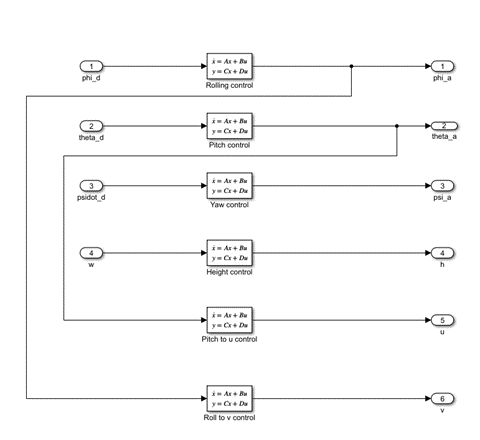
\includegraphics[width=0.8\textwidth]{Images/position_control}
	\caption{Simulink Design Dynamic Model}
	\label{fig:pc}
\end{figure}

\section{Development of Position/Orientation control system:}

Position/Orientation Control System contains two types of state input, one is the target x, y, and z coordinate input and the other is actual x, y and z coordinates of the quadrotor. A reference yaw command is also given into the position controller to ensure that the quadrotor maintains the commanded yaw while operating for the target position.

The target x coordinate is given into a summation block while the actual x orientation of the quadrotor is given to the summation block as feedback. This command is fed into the PD controller, which gives corresponding derivative $\dot{x}$ (i.e., speed along x axis). This derived velocity u is given to the summation block whereas the actual velocity $ u_a $ is given as feedback in the same block. A PD controller is used again which finally gives the derivative $\ddot{x}$ . 

Similarly, target y position and actual y position of the quadrotor is also given into the summation block and then into the PD controller. The output from this PD controller is further given into a summation block where the actual velocity v is given as feedback. This output is then given into the PD controller to get acceleration along y-axis. 

Actual heading angle psi, along with $\ddot{x}$ and $\ddot{y}$ is used to calculate the desired pitch angle and desired roll angle. The following equations [reference no?] are used for this: \\

\left[\begin{array}{c}
	\phi_{d} \\
	\theta_{d}
\end{array}\right]=\left[\begin{array}{cc}
	-\sin \psi & -\cos \psi \\
	\cos \psi & -\sin \psi
\end{array}\right]^{-1} \frac{m}{U_{1}}\left[\begin{array}{l}
	\ddot{x}_{d} \\
	\ddot{y}_{d}
\end{array}\right] \\


Since the derivation of these equations in (reference no) uses small angle approximation, we must ensure that the desired angles $\theta_{d}$ and $\phi_{d}$ are within the limit of –20° and 20°. Therefore, a saturation block is placed at the output of MATLAB function block.   

We also need the desired vertical velocity w and the desired heading rate $\dot{psi$ to be given into the dynamics model of the quadrotor. For this, desired z coordinate and actual z coordinate are given into a summation block and PD controller is used to obtain the desired w velocity. Similarly, actual yaw angle and desired yaw angle along with PD controller are used to obtain heading rate $\dot{psi}$. 
	
\section{Development of Position Estimation:}

For estimating the position of the quadrotor, the output states from the dynamic model i.e., psi, psi, theta, h, u and v, are used. The dynamic model provides information about the actual value of states of the quadrotor. To acquire data regarding the actual x and y coordinated of the quadrotor we integrate the u and v velocities, respectively. The Simulink model of position estimation subsystem is shown in \ref{fig:pe}.

\begin{figure}
	\centering
	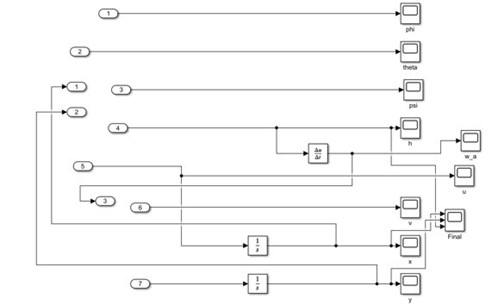
\includegraphics[width=0.8\textwidth]{Images/pe}
	\caption{Position Estimation}
	\label{fig:pe}
\end{figure}
 
 \section{Development of linear simulation model:}
 
 For the development of the linear simulation model, a reference subsystem was created which was used for giving the desired coordinate information to the position controller. The desired pitch and roll angles $ \theta_{d} $ and $\phi_{d}$ along with the heading rate $\dot{psi}$ and desired vertical velocity wd goes into a summation block followed by a PID controller. To this summation block feedback is given of actual orientation of the respective states. 
 
 Further, these values are given into the dynamics model subsystem which is also explained in the previous section. The actual values obtained from the dynamic model are used in the position estimation subsystem to get information about Euler angles, position, and velocities of the quadrotor. 
 
 The reference position subsystem developed in for this project is an If-Else condition block which is used with Action block to activate a particular command for an If-Else condition. The reference command subsystem is shown in the \ref{fig:rp}.
 \begin{figure}
 	\centering
 	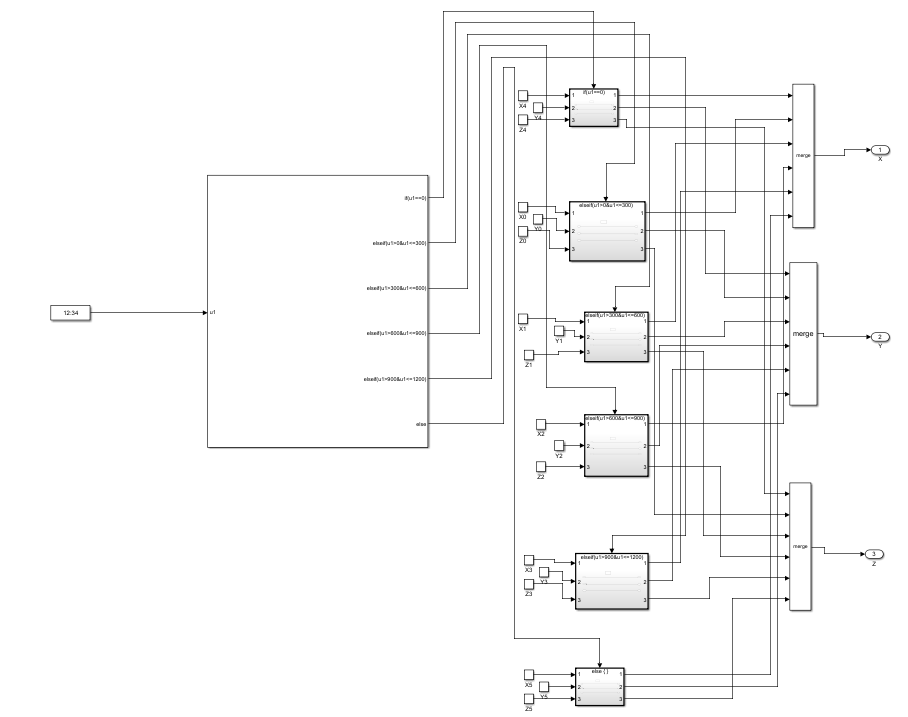
\includegraphics[width=0.8\textwidth]{Images/rp}
 	\caption{Reference Position}
 	\label{fig:rp}
 \end{figure}

The complete linear simulation system that was developed in Simulink is shown in the \ref{fig:cm} 

PID Tuning methods used for this project were Inbuilt PID tuners provided by Simulink. For tuning PD controllers, the following steps were taken:
\begin{enumerate}
	\item Proportional gain Kp was increased until steady oscillations were obtained
	\item Derivate gain Kd was increased until the oscillations were critically damped
\end{enumerate} \\

\begin{figure}
	\centering
	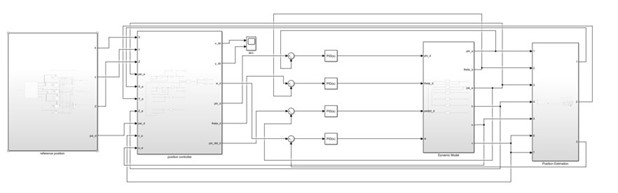
\includegraphics[width=1.1\textwidth]{Images/multirotor}
	\caption{Complete Multirotor Dynamic System}
	\label{fig:cm}
\end{figure}

Total simulation time was taken to be 1500 seconds for the following four maneuvers: \\
\begin{enumerate}
	\item Take off and hover at 2 meters above origin
	\item Fly to the first target (x = 5 m, y = 6 m, h = 4 m) and hover
	\item Fly to the second target (x = -5 m, y = -6 m, h = 4 m) and hover
	\item Return to 2 meters above origin and land
\end{enumerate}

\section{Result}

The quadcopter was successfully able to complete all the given maneuvers for this project. The simulation result, which shows the trajectory of x, y and z coordinates of the quadcopter for 1500 seconds is shown in . 

\begin{figure}
	\centering
	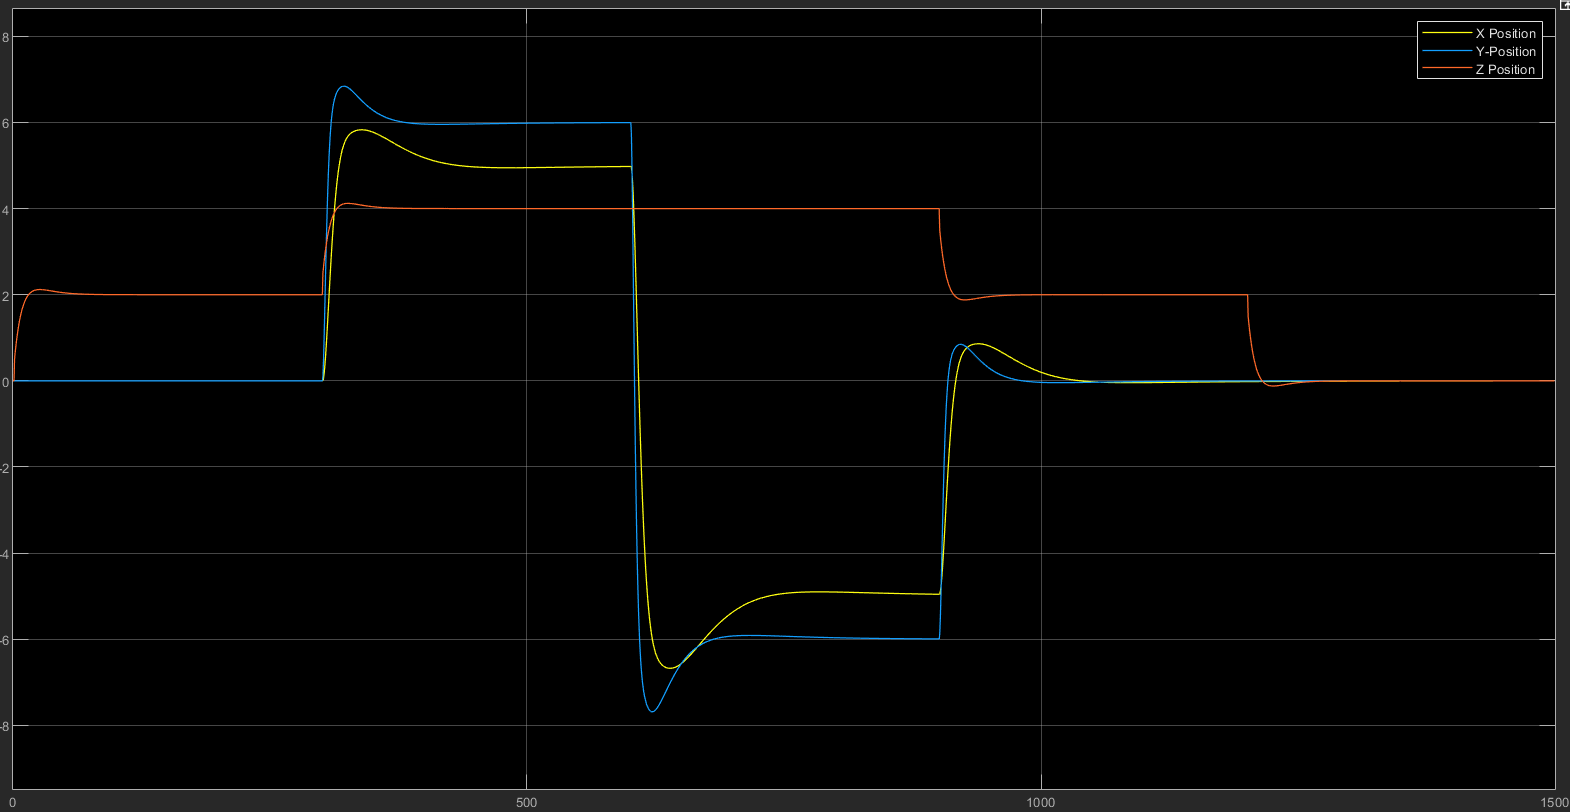
\includegraphics[width=1.1\textwidth]{Images/multirotor_sol}
	\caption{Quadrotor Simulation Solution}
	\label{fig:m_sol}
\end{figure}\\

In the figure the quadcopter is initially at x=0, y=0 and z=0 position, in the first 300 seconds it takes off and hover at x=0 y=0 and z=2 m. Next, the quadcopter reaches to x=5, y=6 and z=4.For the third maneuver it goes from its current position to the target position, x=-5, y=-6 and z=4 and then for the last maneuver is goes from current position to target position of x=0, y=0 and z= 2 and then back to the origin. 